\chapter[TINJAUAN PUSTAKA]{TINJAUAN PUSTAKA}
\sloppy

\section{Analitik Perilaku Konsumen pada Area Komersial}

Analitik perilaku konsumen berbasis visi komputer merupakan teknologi esensial bagi industri ritel fisik untuk memahami pola interaksi pelanggan secara kuantitatif. Tiga metrik utama yang sering diukur meliputi volume kunjungan (\textit{counting}), tingkat kepadatan area (\textit{occupancy}), dan waktu singgah (\textit{dwell time}). Menurut tinjauan sistematis dalam literatur visi komputer, pemanfaatan jaringan multi-kamera di sektor ritel (\textit{smart stores}) diterapkan secara spesifik untuk memetakan arus pergerakan komersial secara efisien tanpa memerlukan identifikasi biometrik eksplisit \cite{fierrosilva2026}. Pemanfaatan data trajektori pelacakan konsumen melalui kamera pengawas memungkinkan pembentukan peta persebaran spasial (\textit{heatmap}) guna mengidentifikasi zona-zona yang paling banyak dikunjungi pembeli di dalam gerai \cite{narvilas2022}.

Pemahaman perilaku konsumen dapat diperdalam lebih lanjut melalui analisis arah tatapan (\textit{gaze estimation}) berbasis pembelajaran mendalam (\textit{deep learning}) untuk mengetahui etalase produk mana yang secara spesifik menarik perhatian pembeli \cite{senarath2022}. Namun demikian, seluruh analisis metrik lanjutan tersebut sangat bergantung pada keandalan sistem tingkat dasar dalam mendeteksi dan melacak pergerakan pelanggan secara konsisten dari waktu ke waktu \cite{shili2024electronics}.

\section{Deteksi Objek (YOLO)}

Algoritma \textit{You Only Look Once} (YOLO) merupakan arsitektur mutakhir dalam deteksi objek berbasis \textit{Convolutional Neural Network} (CNN) yang beroperasi secara waktu nyata. Prinsip kerja YOLO didasarkan pada perlakuan deteksi sebagai masalah regresi tunggal, di mana citra masukan diproses secara langsung untuk memprediksi koordinat kotak pembatas (\textit{bounding box}) beserta probabilitas kelas objek secara simultan. Efisiensi komputasi arsitektur CNN ringan seperti varian YOLO menjadikannya pilihan dominan untuk implementasi praktis di lingkungan komersial cerdas dibandingkan arsitektur berbasis model transformator yang membutuhkan komputasi lebih besar \cite{fierrosilva2026}.

Optimalisasi model YOLO pada sektor ritel telah banyak dieksplorasi, salah satunya melalui pengembangan arsitektur LSR-YOLO yang dirancang ringan namun tetap memiliki presisi tinggi dalam mengenali produk di rak toko \cite{zhao2025}. Modifikasi serupa diterapkan pada varian YOLO teroptimasi untuk mengenali produk ritel berukuran kecil (\textit{small objects}) pada kabinet pajang dengan kondisi pencahayaan minim (\textit{low-light}) \cite{yang2026}. Di sisi implementasi perangkat keras, model deteksi berbasis YOLO juga terbukti dapat diintegrasikan secara efektif dengan sistem mikrokontroler lokal untuk menghasilkan dasbor analitik pelanggan secara waktu nyata \cite{hairurizal2026}. Dalam konteks penelitian ini, YOLO versi terbaru (YOLO11) difungsikan sebagai variabel kontrol konstan pada tahap deteksi agar seluruh variasi performa metrik murni merefleksikan keandalan algoritma pelacakan yang diuji.

\section{Multi-Object Tracking (MOT)}

\textit{Multi-Object Tracking} (MOT) merupakan proses komputasi untuk mengidentifikasi keberadaan target serta mempertahankan lintasan (\textit{trajectory}) dari banyak objek secara berkesinambungan dalam urutan bingkai video (\textit{video frames}).

\subsection{Paradigma Tracking-by-Detection}
Pendekatan yang paling dominan digunakan dalam sistem pelacakan modern adalah paradigma \textit{Tracking-by-Detection} (TbD) \cite{panagos2026}. Dalam implementasi visi komputer, sering kali timbul miskonsepsi bahwa algoritma pendeteksi (seperti YOLO) dan algoritma pelacak (seperti ByteTrack) merupakan dua metode alternatif yang saling menggantikan (pilihan A atau B). Secara fundamental, kedua komponen tersebut berada pada tingkatan fungsi yang berbeda dan bekerja secara komplementer dalam satu rangkaian alur pemrosesan (\textit{pipeline}) berurutan, sebagaimana diilustrasikan pada Gambar~\ref{fig:pipeline_tbd}.

\begin{figure}[htbp]
    \centering
    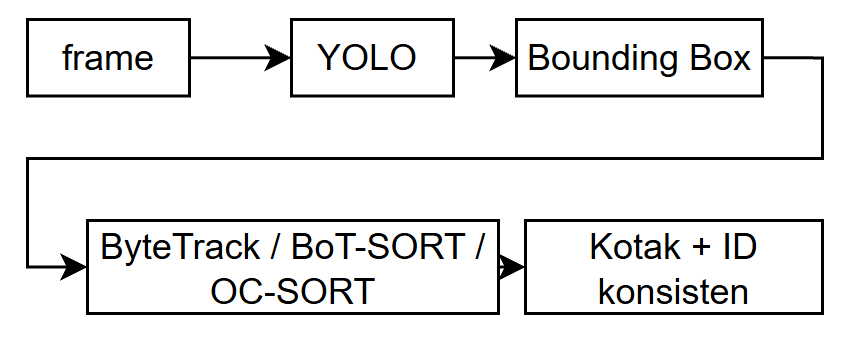
\includegraphics[width=0.8\textwidth]{gambar/Alur Pemrosesan.png}
    \caption{Alur Paradigma \textit{Tracking-by-Detection} pada Pemrosesan Video Ritel}
    \label{fig:pipeline_tbd}
\end{figure}

Modul detektor hanya bertugas melokalisasi koordinat keberadaan objek (\textit{bounding box}) pada setiap bingkai secara independen tanpa memiliki memori temporal terhadap riwayat bingkai sebelumnya. Sebaliknya, modul pelacak (\textit{tracker}) tidak memiliki kapabilitas untuk mendeteksi fitur objek langsung dari piksel mentah; fungsinya adalah menerima sekumpulan kotak deteksi dari detektor untuk kemudian melakukan asosiasi data (\textit{data association}) antar-bingkai, memprediksi perpindahan posisi spasial menggunakan estimasi gerak, serta mempertahankan nomor identitas unik (\textit{tracking ID}) dari setiap individu. Oleh karena itu, penggantian YOLO secara langsung dengan ByteTrack secara teknis tidak dapat dilakukan karena modul pelacak selalu mensyaratkan adanya modul deteksi di bawahnya.

\subsection{Tantangan Oklusi dan Fragmentasi Identitas (Identity Churn)}
Asosiasi data temporal antar-bingkai menghadapi tantangan besar pada skenario dunia nyata, terutama yang diakibatkan oleh variasi pencahayaan, kepadatan kerumunan, dan fenomena oklusi visual \cite{fierrosilva2026}. Oklusi terjadi ketika pandangan kamera terhadap target terhalang oleh partisi gerai, barang bawaan, maupun oleh pengunjung lain yang melintas di depannya \cite{panagos2026, mendes2023multi}.

Saat target tertutup secara visual, detektor gagal menghasilkan kotak deteksi untuk beberapa bingkai. Ketika target tersebut kembali terlihat, modul pelacak standar kerap gagal menautkan target tersebut ke riwayat lintasannya yang lama dan justru memberikan nomor identitas baru. Fenomena ini disebut sebagai pergantian identitas (\textit{identity switch}) atau fragmentasi identitas (\textit{ID churn}) \cite{fierrosilva2026}. Fenomena ini merusak validitas penghitungan metrik analitik bisnis secara signifikan; sebagai contoh, satu orang pelanggan yang berdiri di depan rak display selama lima menit dapat tercatat secara keliru sebagai tiga pelanggan berbeda dengan rata-rata waktu singgah (\textit{dwell time}) yang jauh lebih singkat dari kondisi riil.

\subsection{Algoritma Pelacakan Objek Kontemporer}
Untuk mengatasi kelemahan asosiasi data akibat oklusi, berbagai algoritma pelacakan modern dikembangkan dengan mekanisme inferensi yang berbeda:
\begin{enumerate}
    \item \textbf{ByteTrack}: Mengajukan metode asosiasi BYTE yang memanfaatkan kotak deteksi dengan nilai kepercayaan rendah selain deteksi berskor tinggi. Strategi ini terbukti efektif mempertahankan kesinambungan lintasan target saat mengalami oklusi sebagian tanpa menambah beban komputasi ekstraksi fitur kenampakan.
    \item \textbf{BoT-SORT}: Merupakan penyempurnaan dari arsitektur SORT dengan mengintegrasikan kompensasi pergerakan kamera (\textit{Camera Motion Compensation}) serta estimasi kecepatan yang lebih stabil pada filter Kalman untuk memperkuat akurasi lokalisasi spasial.
    \item \textbf{OC-SORT}: \textit{Observation-Centric SORT} dirancang khusus untuk memulihkan lintasan setelah oklusi berkepanjangan dengan mengurangi akumulasi galat linier pada filter Kalman konvensional melalui pembaruan observasi mundur (\textit{observation-centric recovery}).
    \item \textbf{Deep OC-SORT}: Merupakan varian lanjutan dari OC-SORT yang mengombinasikan pelacakan berbasis observasi dengan modul ekstraksi fitur kenampakan (\textit{appearance embeddings/Re-ID}) guna memperkuat keandalan asosiasi identitas saat terjadi oklusi durasi panjang di area yang padat.
\end{enumerate}

\section{Metrik Evaluasi Pelacakan Standar Akademik}

Secara konvensional di lingkungan penelitian akademik, performa sistem MOT dievaluasi menggunakan tolok ukur standar berbasis matriks kesalahan:
\begin{enumerate}
    \item \textbf{MOTA (\textit{Multiple Object Tracking Accuracy})}: Mengukur akurasi pelacakan secara agregat dengan mengombinasikan kesalahan deteksi positif palsu (\textit{false positives}), deteksi tidak terdeteksi (\textit{false negatives}), dan frekuensi pergantian identitas (\textit{identity switches}). Karena formulasinya didominasi oleh jumlah kesalahan lokalisasi, nilai MOTA cenderung lebih sensitif terhadap performa detektor dibandingkan kemampuan mempertahankan identitas objek jangka panjang.
    \item \textbf{IDF1 (\textit{Identification F1-Score})}: Merupakan nilai rata-rata harmonik antara presisi identifikasi dan \textit{recall} identifikasi. Berbeda dengan MOTA, IDF1 dirancang secara spesifik untuk mengukur sejauh mana algoritma pelacak mampu mempertahankan lintasan identitas target yang konsisten sepanjang waktu pengamatan.
\end{enumerate}

\section{Penelitian Terkait}

Penerapan visi komputer di sektor ritel telah berkembang pesat untuk menjawab kebutuhan analitik otomatis. Penggunaan kombinasi algoritma YOLOv5 dan DeepSORT telah dibuktikan mampu memantau interaksi pelanggan secara akurat di depan rak pajang, yang berkorelasi positif terhadap evaluasi penataan produk serta peningkatan rasio konversi penjualan (\textit{conversion rates}) \cite{shili2024algorithms, shili2024electronics}. Pemanfaatan lintasan koordinat dari model serupa juga terbukti efektif dalam memetakan kepadatan pengunjung toko ke dalam format peta sebaran komersial \cite{narvilas2022}.

Di ranah pengembangan algoritma pelacakan, berbagai strategi komputasi terus diusulkan guna mengatasi kendala hilangnya identitas akibat oklusi visual. Pemanfaatan karakteristik historis lintasan pergerakan target (\textit{trajectory data}) telah dikembangkan untuk menstabilkan re-identifikasi subjek pada jaringan multi-kamera yang memiliki area tanpa tumpang-tindih sudut pandang \cite{mendes2023multi}. Pada lingkungan belanja yang padat, kerangka kerja pelacakan yang mempertimbangkan atribut demografi diusulkan dengan memasukkan konsistensi estimasi gender dan kelompok usia sebagai variabel pembobot asosiasi temporal guna meminimalkan tertukarnya identitas antar-pelanggan yang berpapasan dekat \cite{panagos2026}. Sementara itu, pendekatan mutakhir seperti ReTrackVLM mengintegrasikan representasi visual-bahasa dengan modul Re-ID untuk mewujudkan asosiasi identitas yang tangguh dalam kondisi tanpa pelatihan awal (\textit{zero-shot tracking}) \cite{bayraktar2025retrackvlm}. Seluruh kemajuan arsitektur tersebut membuktikan bahwa integrasi model gerak temporal dan penalaran spasial merupakan kunci utama dalam menjaga korelasi identitas objek pada pemantauan visual \cite{fierrosilva2026}.

Berdasarkan telaah literatur mutakhir, mayoritas penelitian analitik ritel saat ini terbagi ke dalam dua fokus utama: penyederhanaan beban komputasi model deteksi agar dapat berjalan pada perangkat berdaya rendah \cite{zhao2025, yang2026}, atau peningkatan skor evaluasi teoretis pada tolak ukur akademik seperti MOTA dan IDF1 \cite{panagos2026, bayraktar2025retrackvlm}. Namun, sangat jarang ditemukan penelitian yang secara empiris mengkaji apakah tingginya pencapaian metrik evaluasi akademik tersebut berkorelasi langsung dengan ketepatan penghitungan metrik perilaku konsumen di lapangan—khususnya pada margin galat estimasi waktu singgah (\textit{dwell time}) dan waktu tunggu antrean akibat fenomena pergantian identitas (\textit{ID churn}). Penelitian tugas akhir ini hadir untuk menjembatani kesenjangan tersebut melalui pengujian performa empat algoritma pelacakan modern (\textit{ByteTrack, BoT-SORT, OC-SORT, Deep OC-SORT}) menggunakan detektor YOLO11 konstan secara langsung terhadap data operasional ritel aktual.